\documentclass[11pt, a4paper]{article}
\usepackage{pdfpages}
\usepackage{parallel}
\usepackage[T2A]{fontenc}
\usepackage{ucs}
\usepackage[utf8x]{inputenc}
\usepackage[polish,english,russian]{babel}
\usepackage{hyperref}
\usepackage{rotating}
\usepackage[inner=2cm,top=1.8cm,outer=2cm,bottom=2.3cm,nohead]{geometry}
\usepackage{listings}
\usepackage{graphicx}
\usepackage{wrapfig}
\usepackage{longtable}
\usepackage{indentfirst}
\usepackage{array}
\usepackage{tikzsymbols}
\usepackage{soul}
\usepackage[ruled,vlined]{algorithm2e}
%\counterwithout{figure}{section} 

\usepackage{url}
\makeatletter
\g@addto@macro{\UrlBreaks}{\UrlOrds}
\makeatother

\newcolumntype{P}[1]{>{\raggedright\arraybackslash}p{#1}}
\frenchspacing
\usepackage{fixltx2e} %text sub- and superscripts
\usepackage{icomma} % коскі ў матэматычным рэжыме
\PreloadUnicodePage{4}

\newcommand{\longpage}{\enlargethispage{\baselineskip}}
\newcommand{\shortpage}{\enlargethispage{-\baselineskip}}

\def\switchlang#1{\expandafter\csname switchlang#1\endcsname}
\def\switchlangbe{
\let\saverefname=\refname%
\def\refname{Літаратура}%
\def\figurename{Іл.}%
}
\def\switchlangen{
\let\saverefname=\refname%
\def\refname{References}%
\def\figurename{Fig.}%
}
\def\switchlangru{
\let\saverefname=\refname%
\let\savefigurename=\figurename%
\def\refname{Литература}%
\def\figurename{Рис.}%
}

\hyphenation{admi-ni-stra-tive}
\hyphenation{ex-pe-ri-ence}
\hyphenation{fle-xi-bi-li-ty}
\hyphenation{Py-thon}
\hyphenation{ma-the-ma-ti-cal}
\hyphenation{re-ported}
\hyphenation{imp-le-menta-tions}
\hyphenation{pro-vides}
\hyphenation{en-gi-neering}
\hyphenation{com-pa-ti-bi-li-ty}
\hyphenation{im-pos-sible}
\hyphenation{desk-top}
\hyphenation{elec-tro-nic}
\hyphenation{com-pa-ny}
\hyphenation{de-ve-lop-ment}
\hyphenation{de-ve-loping}
\hyphenation{de-ve-lop}
\hyphenation{da-ta-ba-se}
\hyphenation{plat-forms}
\hyphenation{or-ga-ni-za-tion}
\hyphenation{pro-gramming}
\hyphenation{in-stru-ments}
\hyphenation{Li-nux}
\hyphenation{sour-ce}
\hyphenation{en-vi-ron-ment}
\hyphenation{Te-le-pathy}
\hyphenation{Li-nux-ov-ka}
\hyphenation{Open-BSD}
\hyphenation{Free-BSD}
\hyphenation{men-ti-on-ed}
\hyphenation{app-li-ca-tion}

\def\progref!#1!{\texttt{#1}}
\renewcommand{\arraystretch}{2} %Іначай формулы ў матрыцы зліпаюцца з лініямі
\usepackage{array}

\def\interview #1 (#2), #3, #4, #5\par{

\section[#1, #3, #4]{#1 -- #3, #4}
\def\qname{LVEE}
\def\aname{#1}
\def\q ##1\par{{\noindent \bf \qname: ##1 }\par}
\def\a{{\noindent \bf \aname: } \def\qname{L}\def\aname{#2}}
}

\def\interview* #1 (#2), #3, #4, #5\par{

\section*{#1\\{\small\rm #3, #4. #5}}
\ifx\ParallelWhichBox\undefined%
    \addcontentsline{toc}{section}{#1, #3, #4}%
\else%
\ifnum\ParallelWhichBox=0%
    \addcontentsline{toc}{section}{#1, #3, #4}%
\fi\fi%

\def\qname{LVEE}
\def\aname{#1}
\def\q ##1\par{{\noindent \bf \qname: ##1 }\par}
\def\a{{\noindent \bf \aname: } \def\qname{L}\def\aname{#2}}
}

\newcommand{\interviewfooter}[1]{
\vskip 1em
\noindent \textit{#1}
}

\switchlang{en}
\begin{document}

\title{1998 "--- Apple Puck Mouse}
\date{}
\maketitle
\selectlanguage{english}
The Apple USB mouse, often called the “puck” because of its unusual shape, was developed by Apple in 1998. It was the first commercially released Apple mouse with a USB connection rather than the Apple ADB bus. Many reviewers criticized this mouse for its lack of ergonomic design.

\begin{figure}[h]
    \centering
    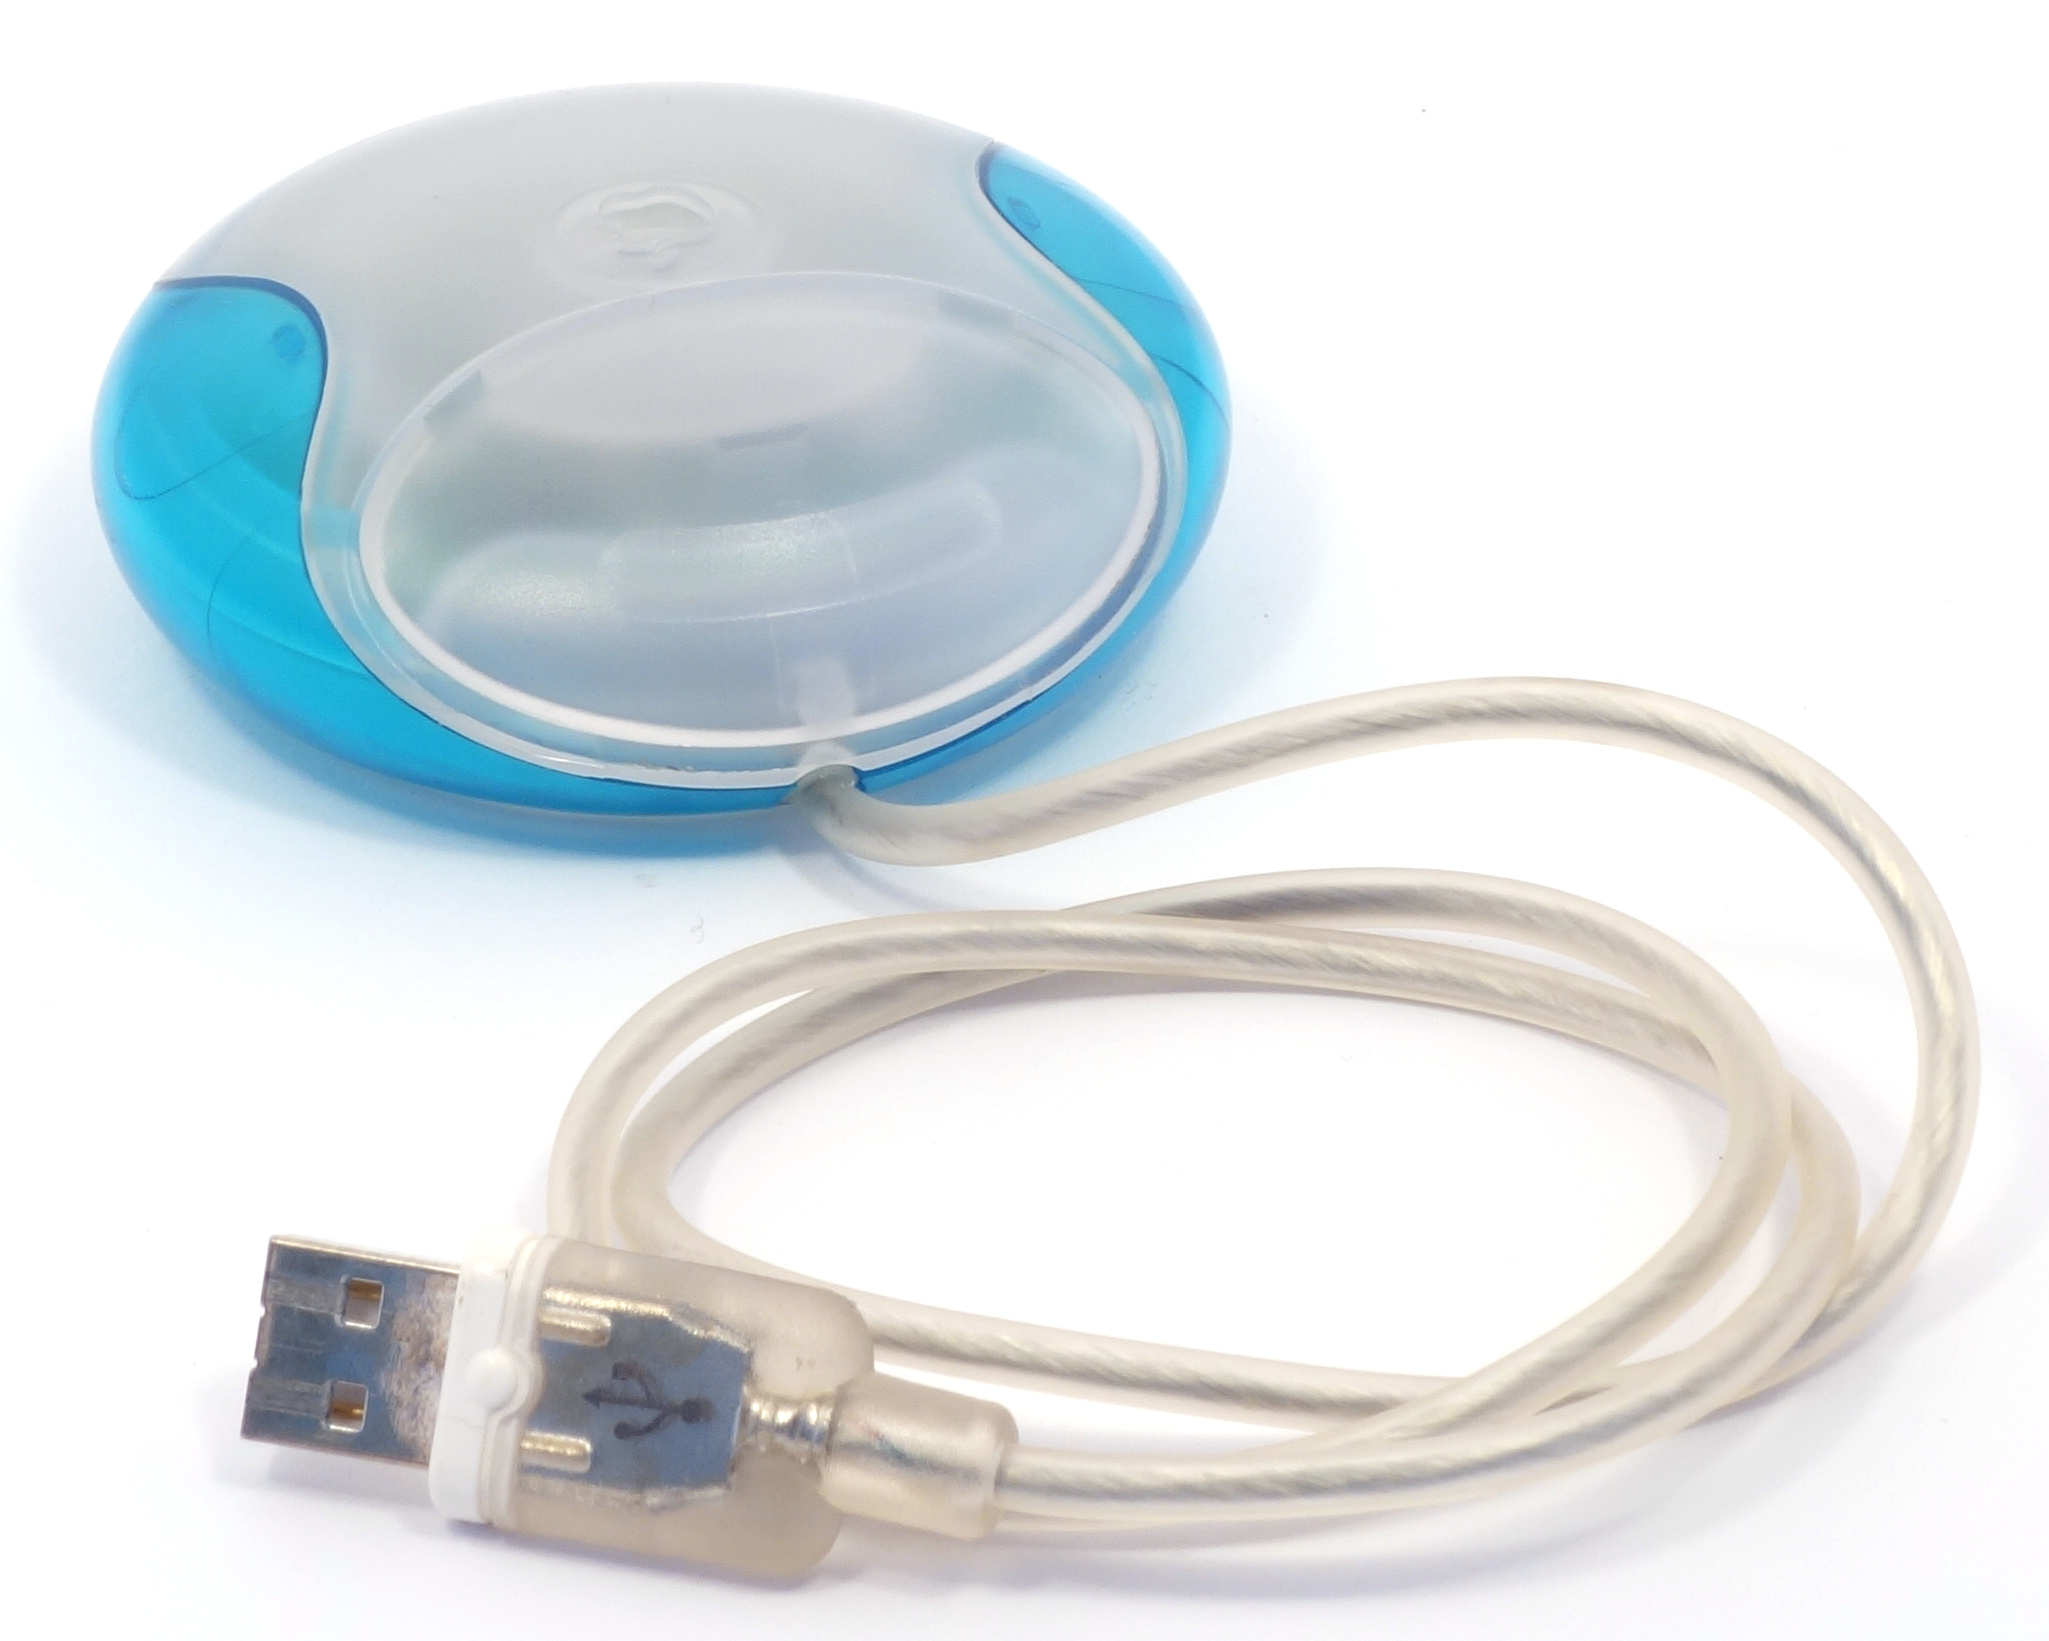
\includegraphics[scale=0.8]{1998_apple_puck/apple60.jpg}
    \caption{Apple Puck Mouse}
    \label{fig:pic}
\end{figure}

Unlike most manipulators, this mouse has a round shape, and it also has one button located at the top, like previous Apple mice. At the same time, the mouse has a gap between the button and the body, showing exactly where the user should press \cite{Apple}.

\begin{figure}[h]
    \centering
    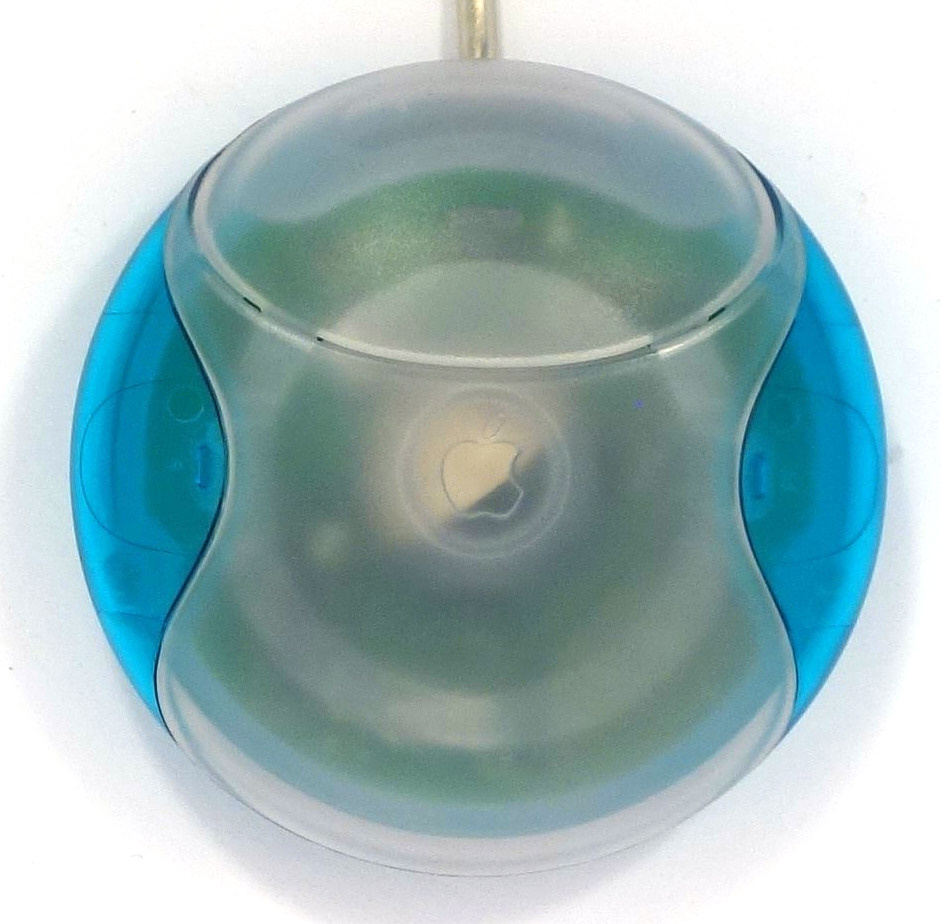
\includegraphics[scale=0.65]{1998_apple_puck/appleup60.jpg}
    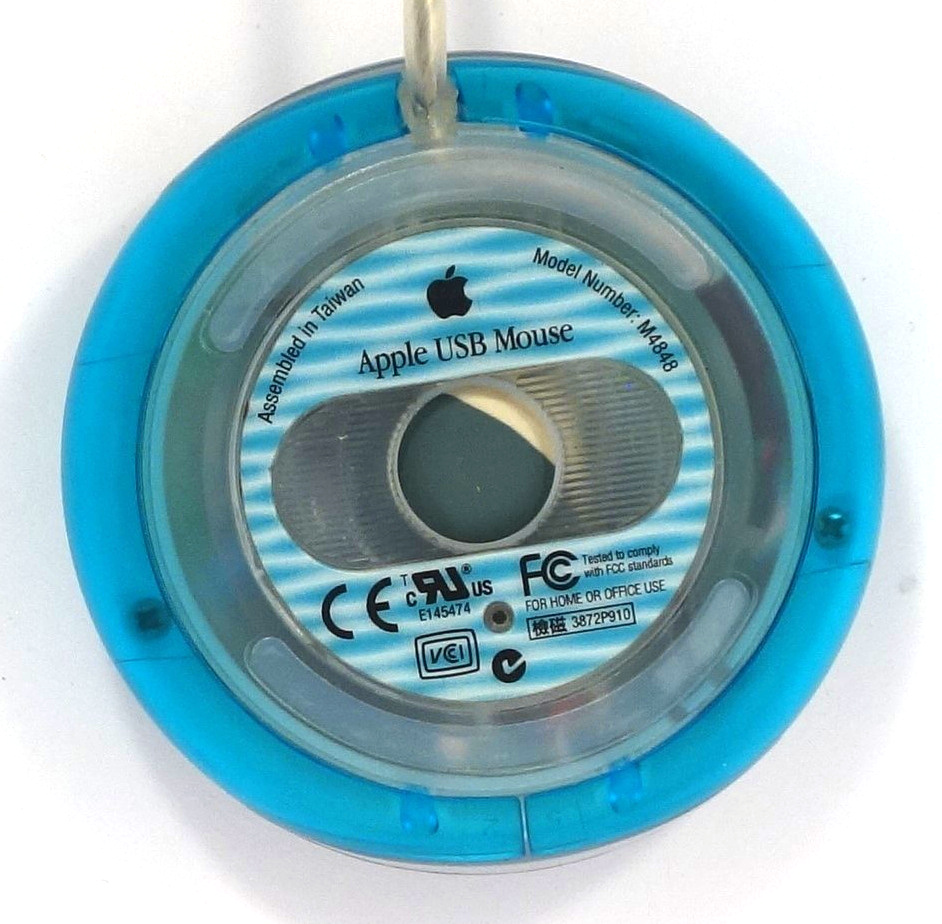
\includegraphics[scale=0.65]{1998_apple_puck/appledown60.jpg}
    \caption{Apple Puck Mouse, top and bottom views}
    \label{fig:top}
\end{figure}

The round shape of the mouse has been considered inconvenient by the community due to the small size of this particular mouse and the tendency to rotate when used.
Also due to the small size, moving the mouse actually required a lot more finger movement and less wrist movement compared to larger mice (figure \ref{fig:size}, \ref{fig:hand}).

\begin{figure}[h]
    \centering
    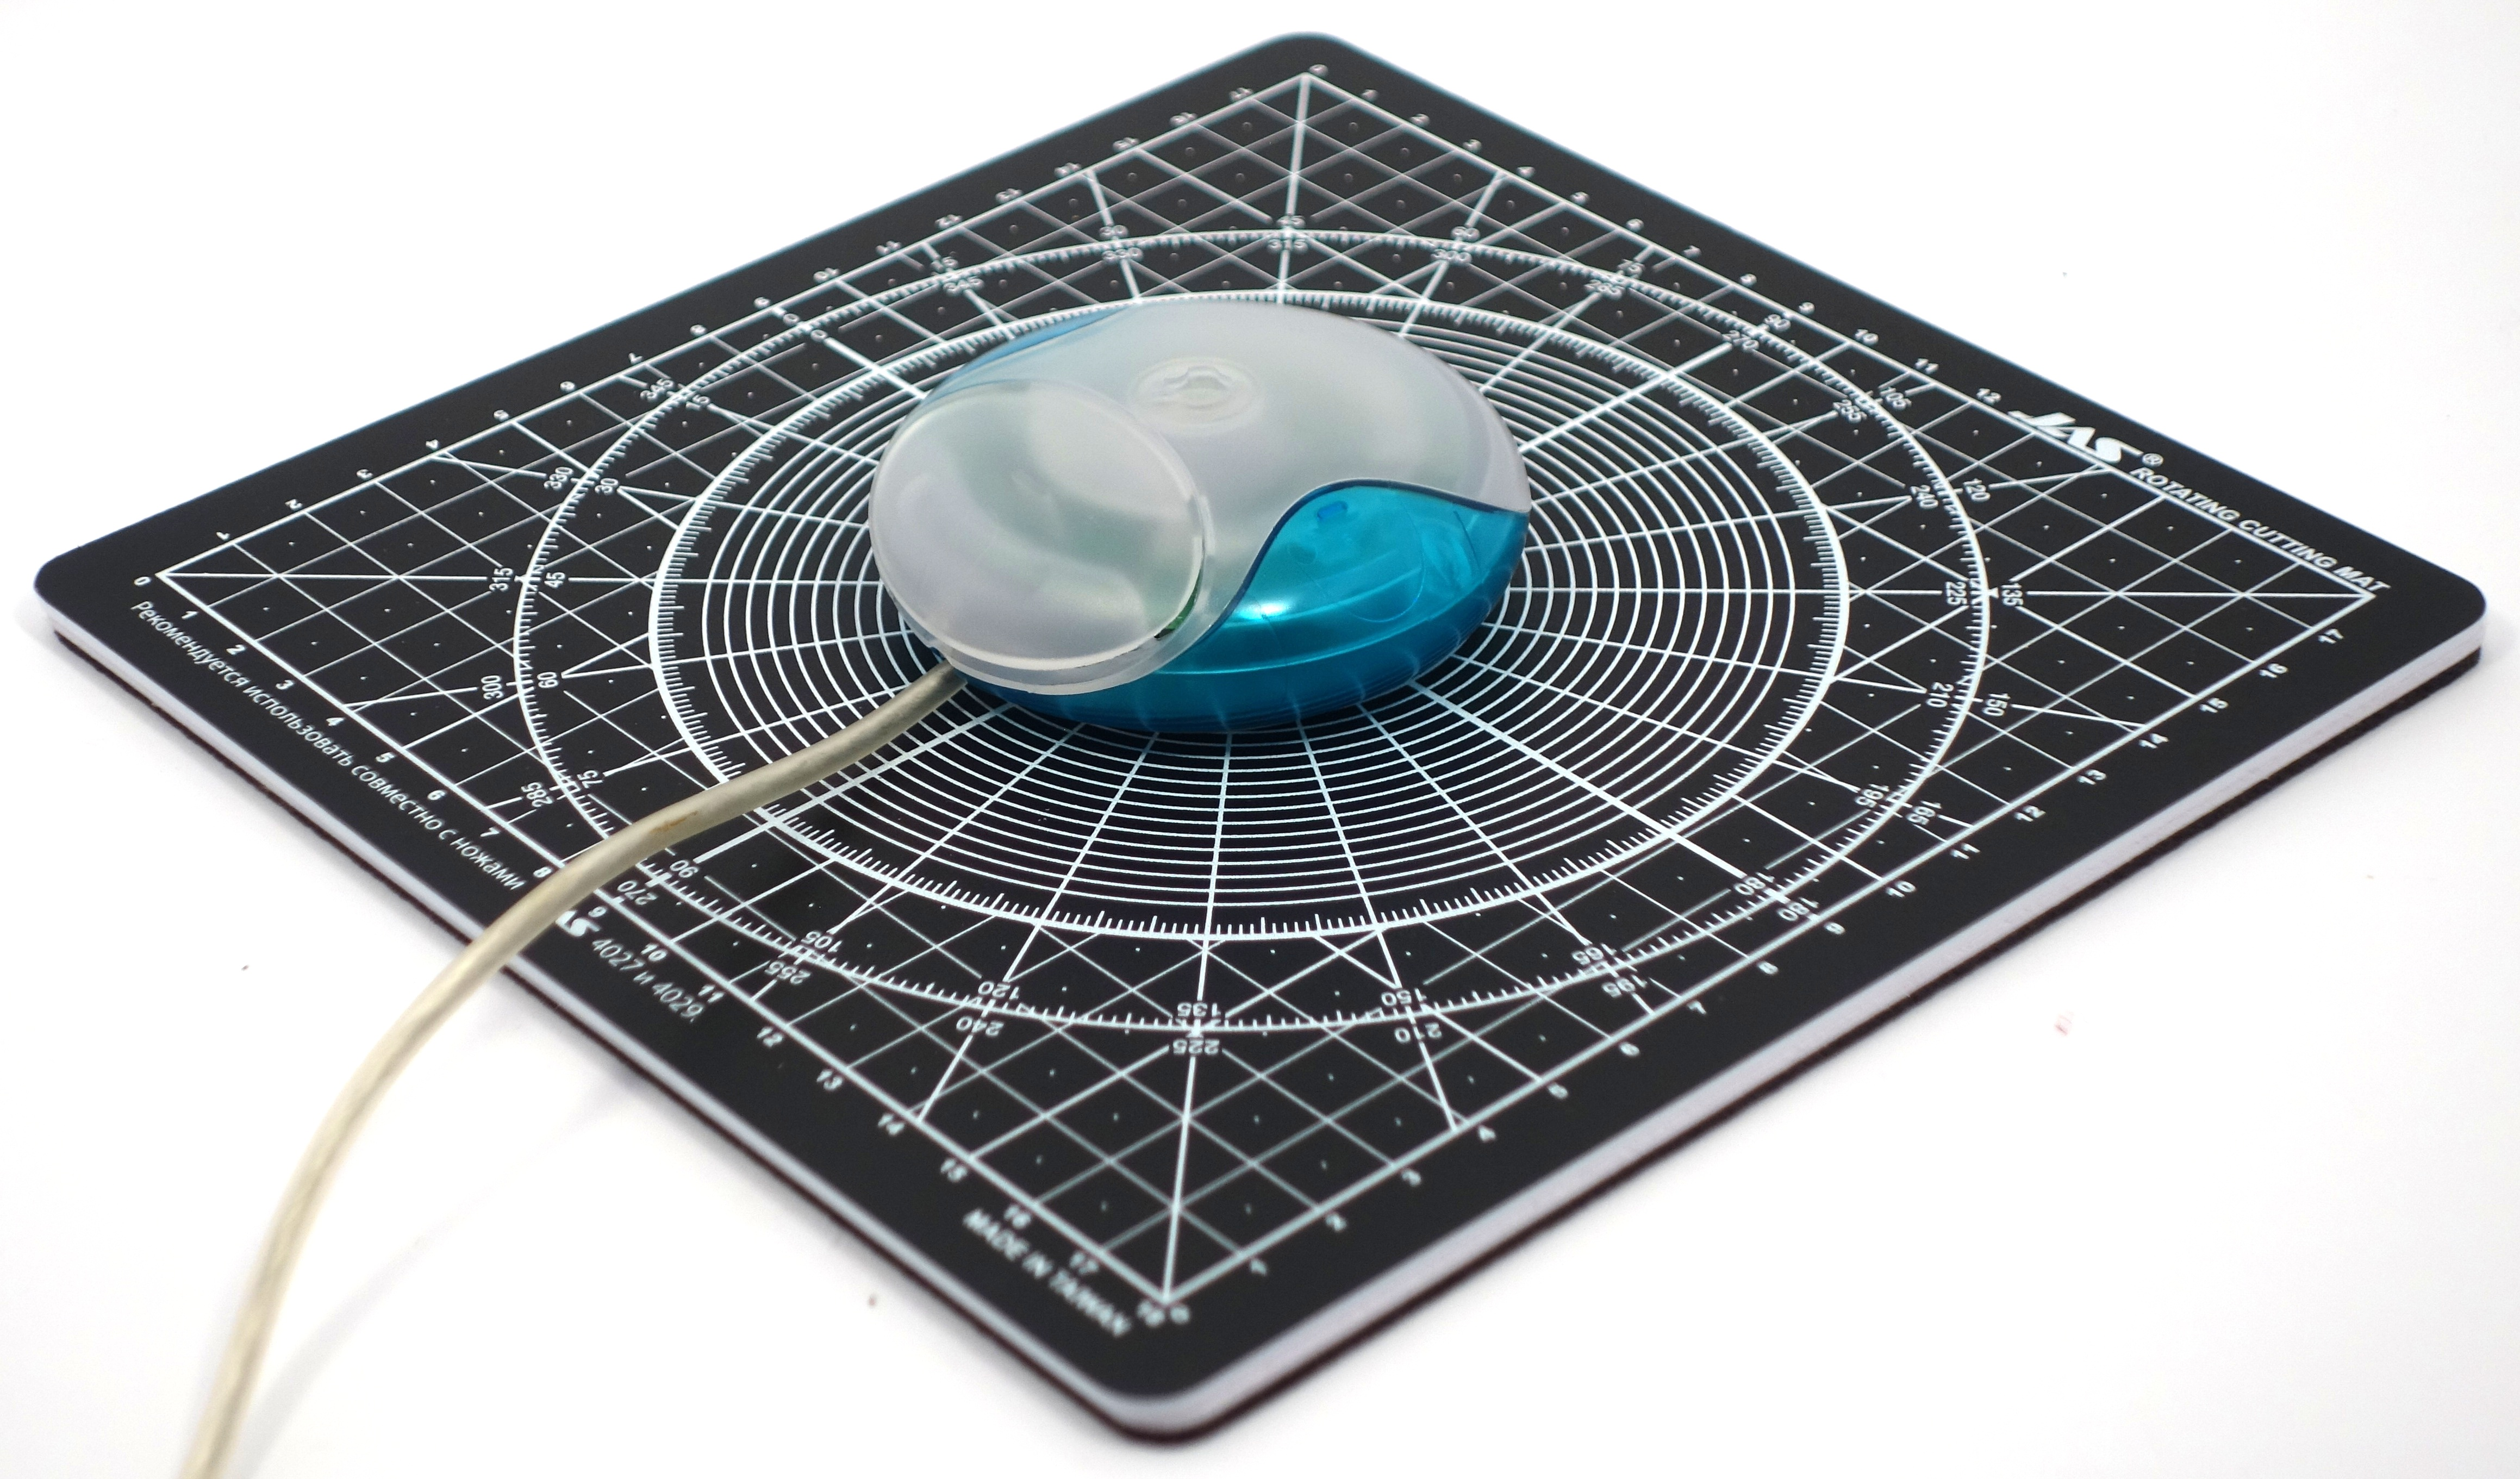
\includegraphics[scale=0.4]{1998_apple_puck/appleset60.jpg}
    \caption{Apple Puck Mouse on a graduated pad with a grid step of 1~cm}
    \label{fig:size}
\end{figure}

\begin{figure}[h]
    \centering
    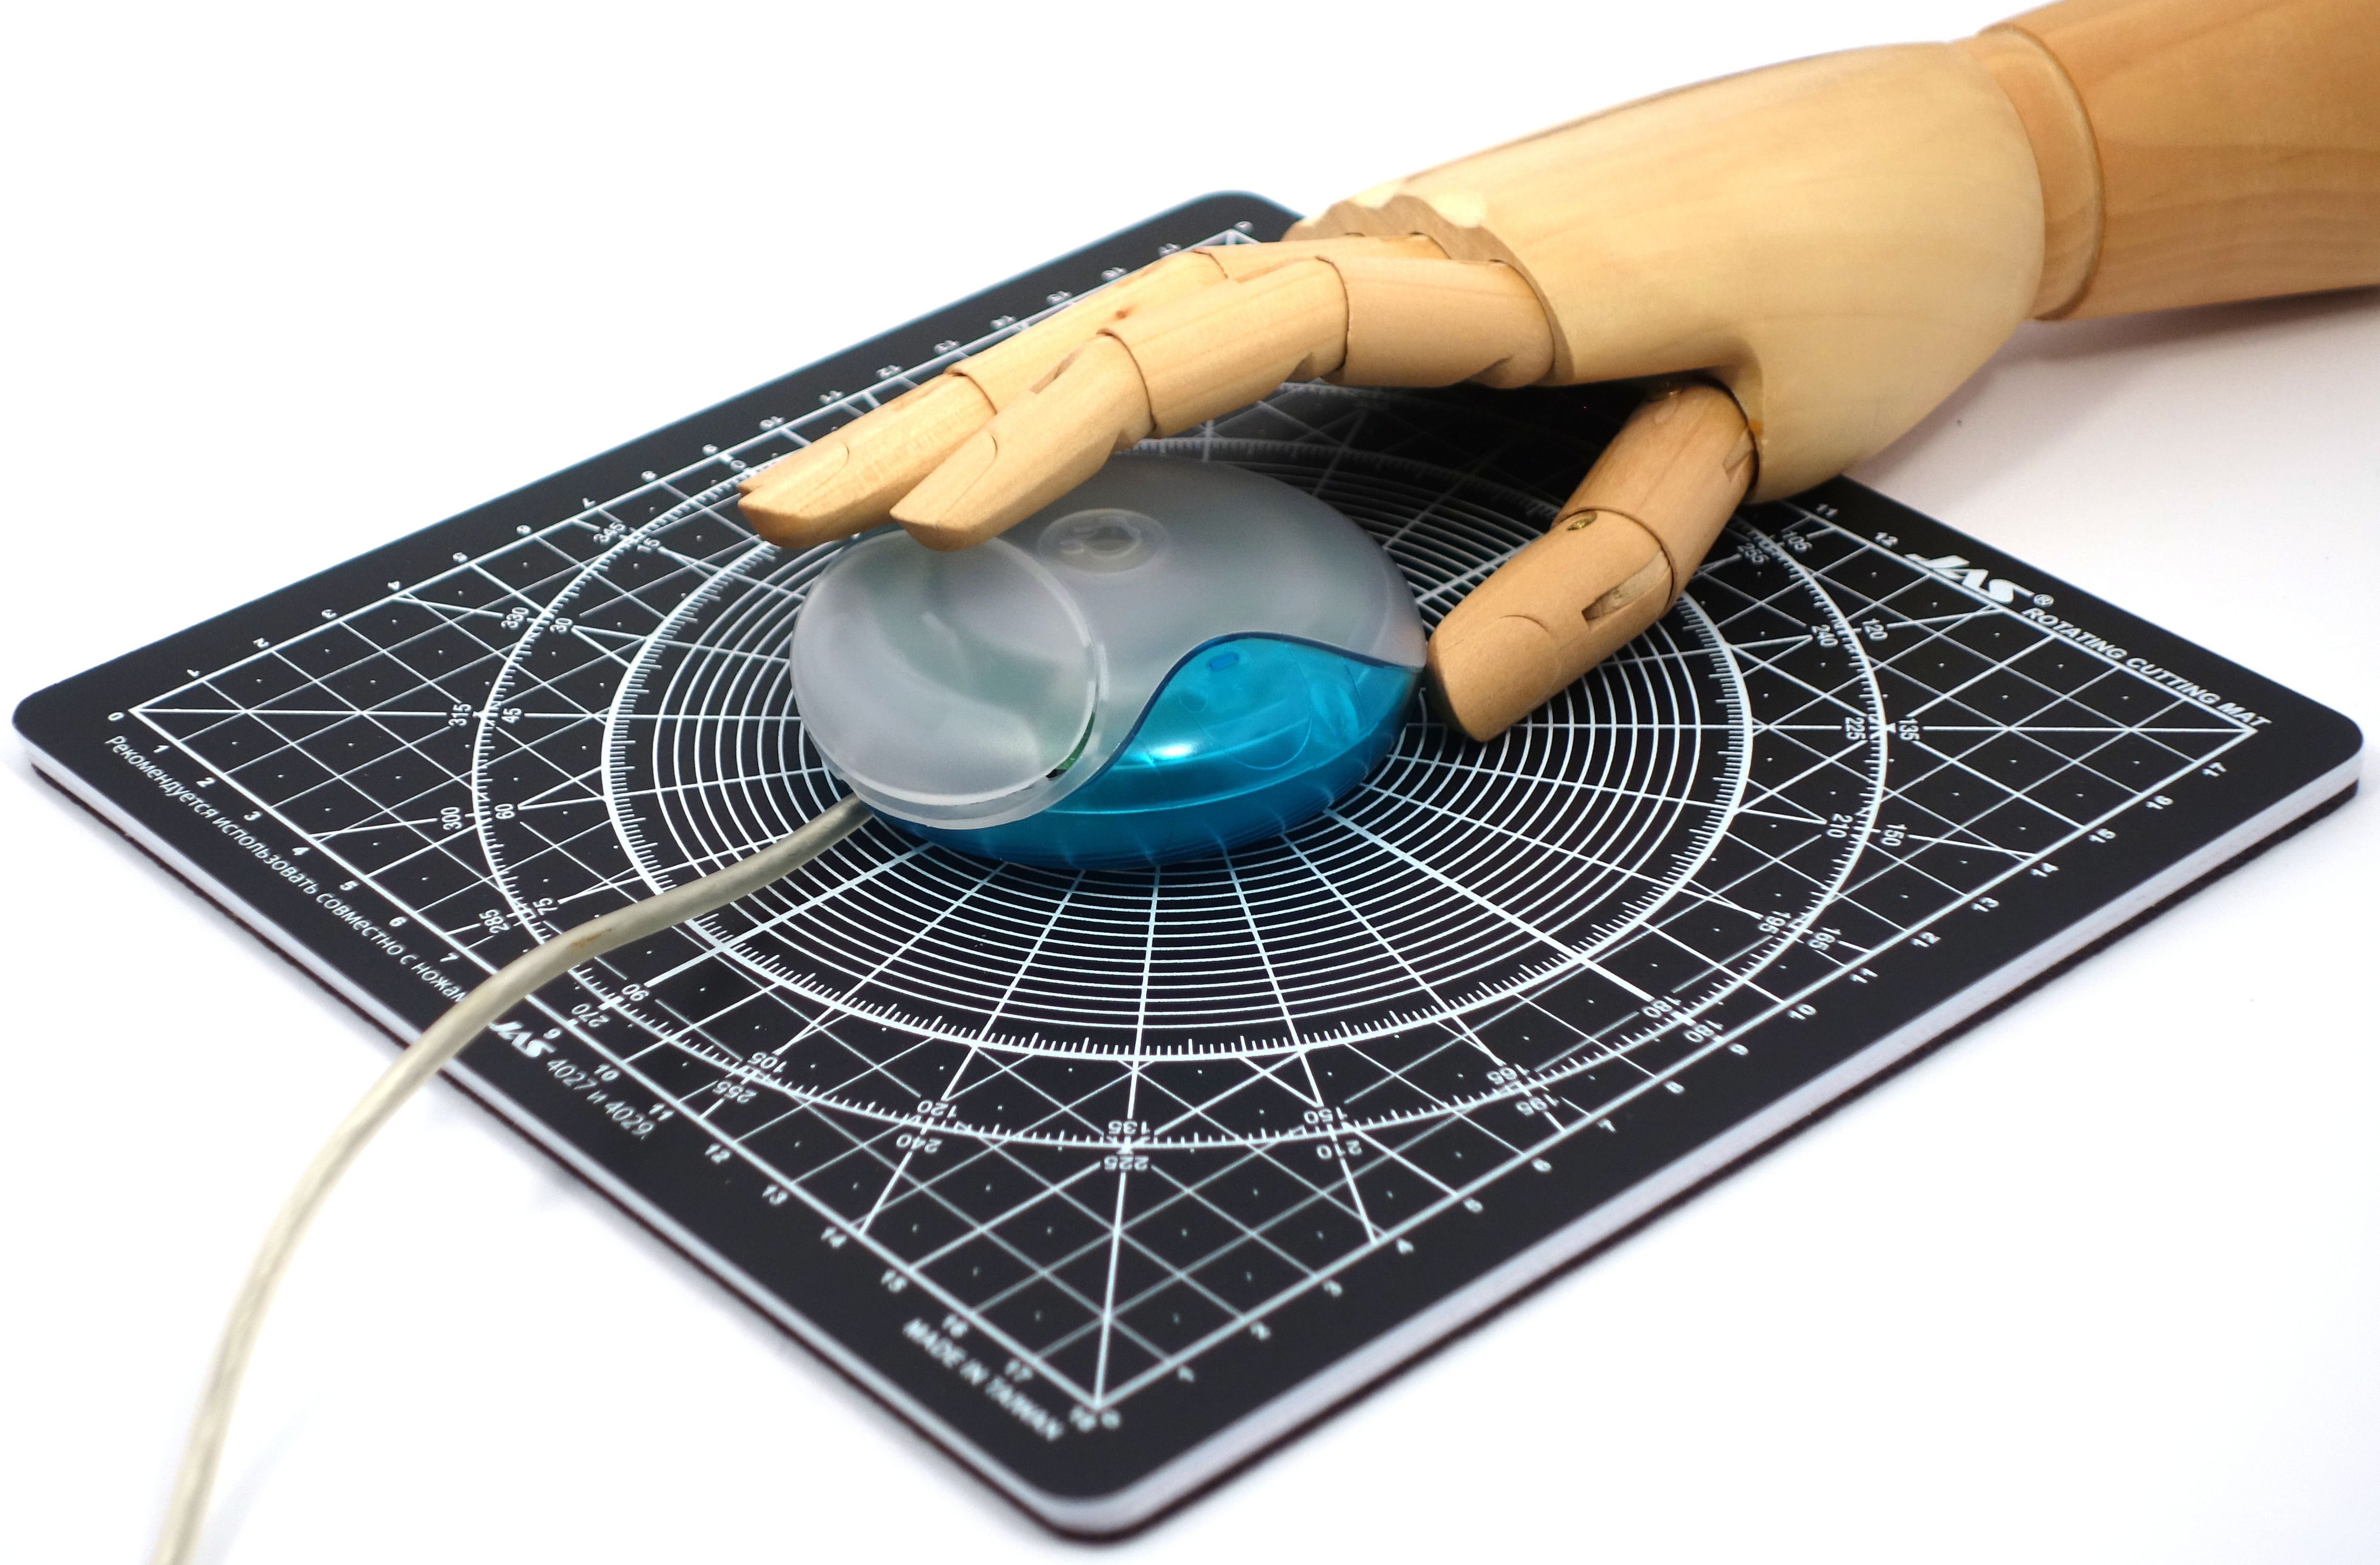
\includegraphics[scale=0.4]{1998_apple_puck/appleset62.jpg}
    \caption{Apple Puck Mouse with a human hand model}
    \label{fig:hand}
\end{figure}

This was the main reason for the success of overlay adapters, such as the iCatch Mouse Adapter \cite{icatch}, which gave the mouse a more elongated shape (figure \ref{fig:addon}).

\begin{figure}[h]
    \centering
    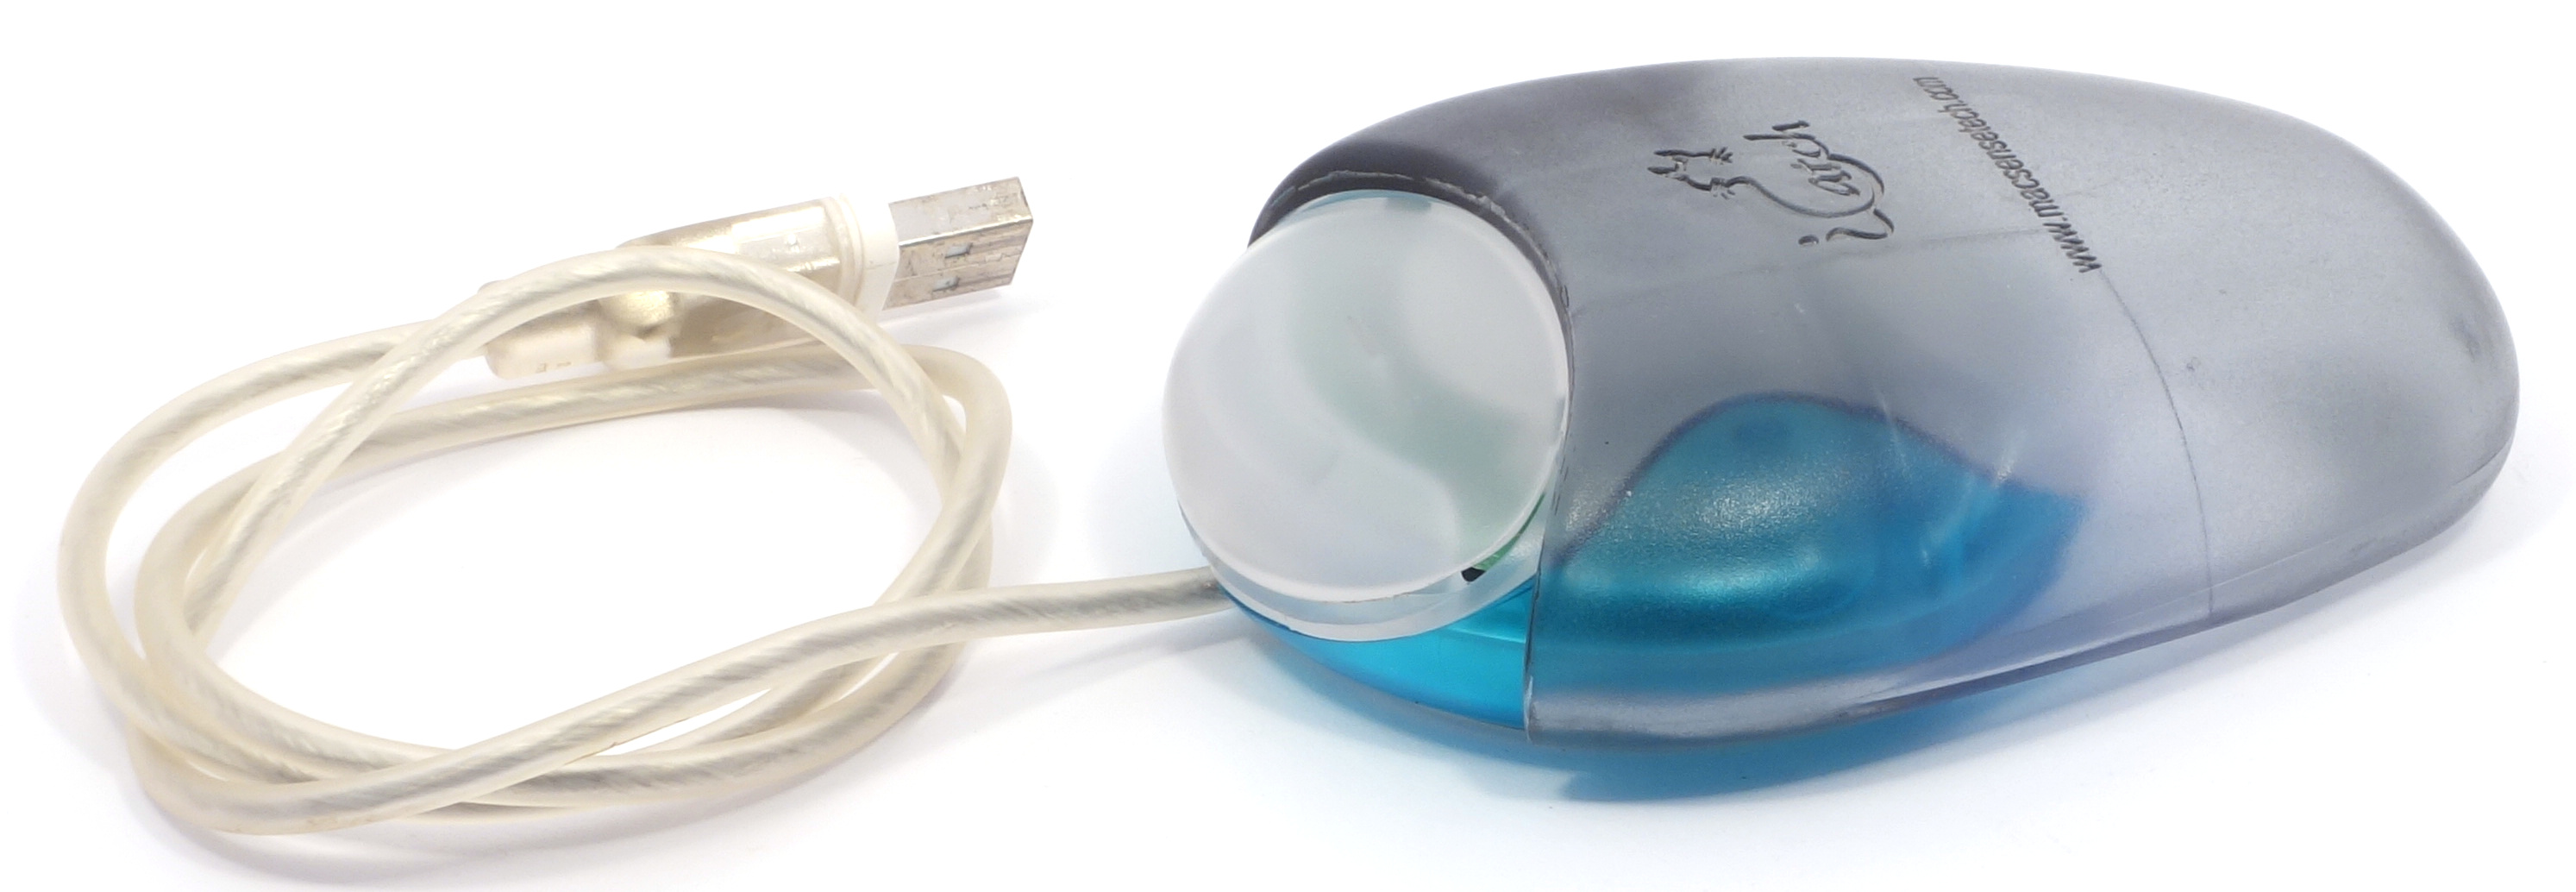
\includegraphics[scale=0.45]{1998_apple_puck/apple63.jpg}
    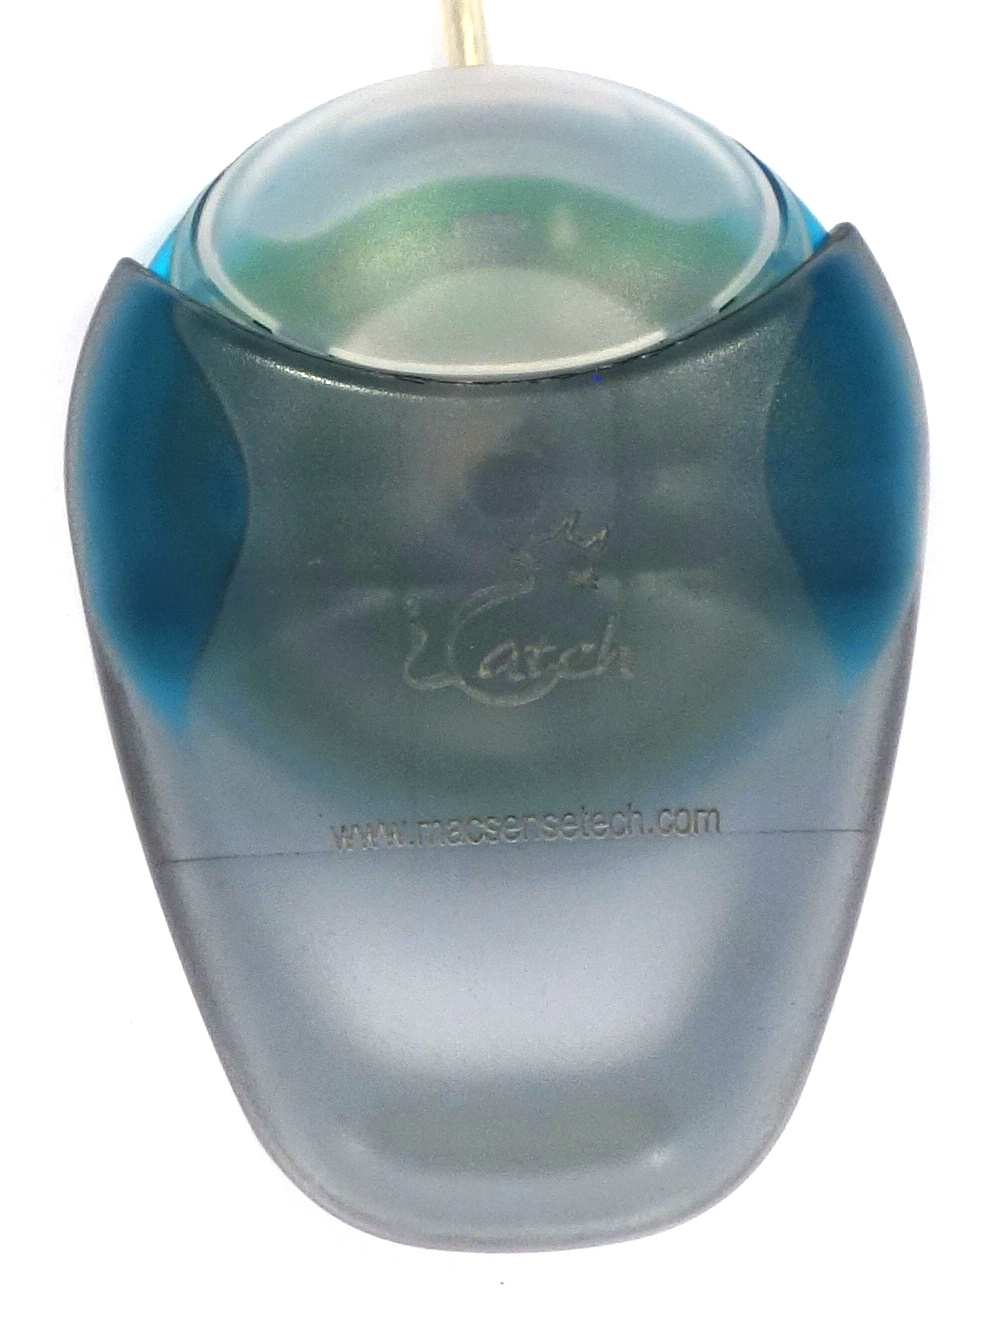
\includegraphics[scale=0.45]{1998_apple_puck/appleup63.JPG}
    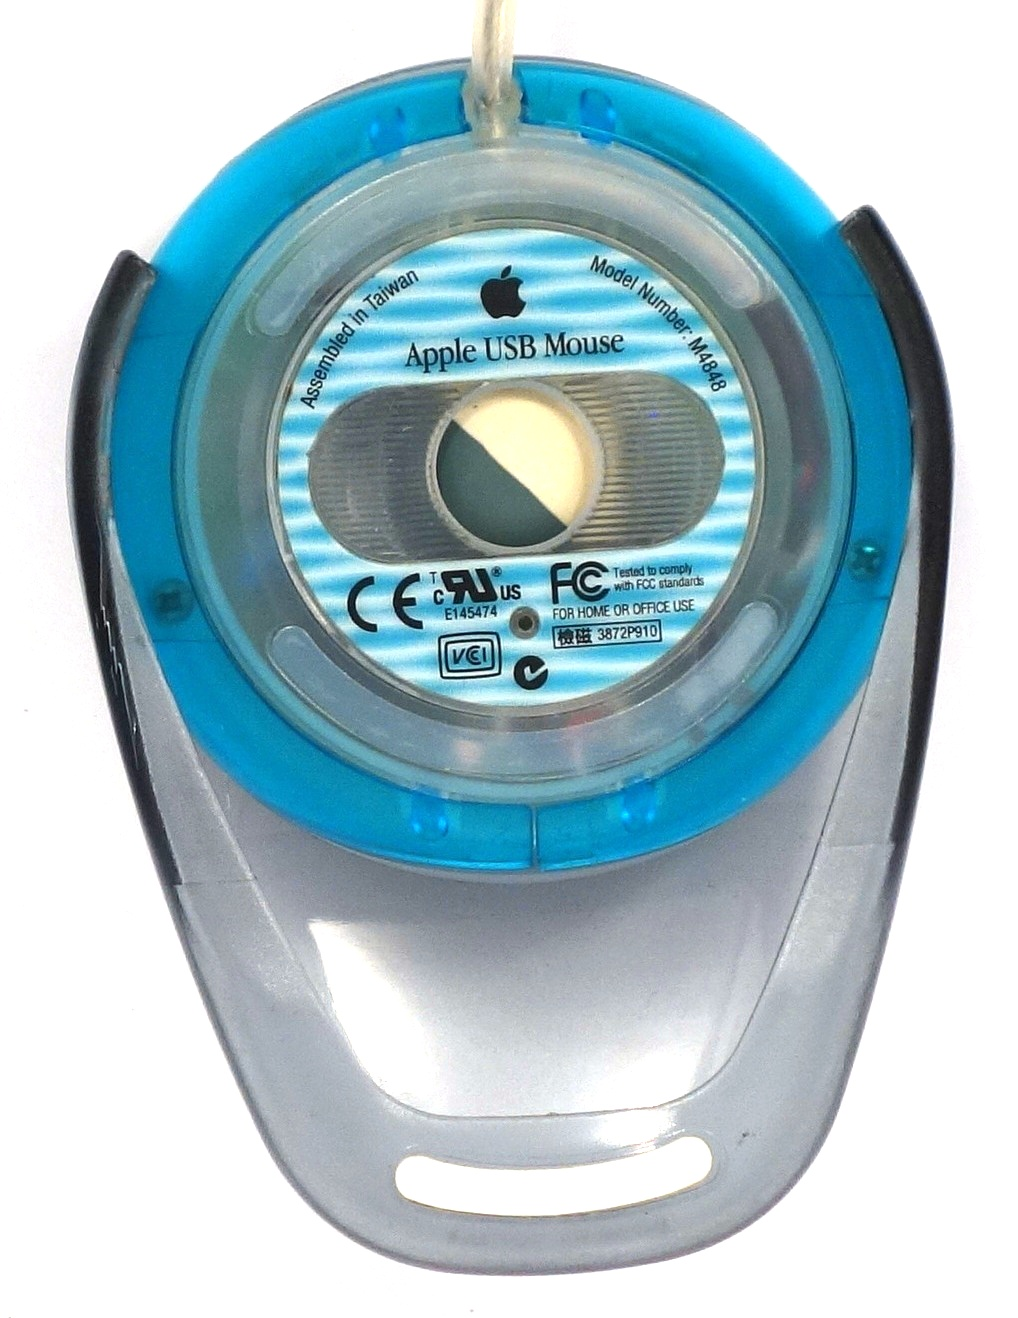
\includegraphics[scale=0.45]{1998_apple_puck/appledown63.JPG}
    \caption{Apple Puck Mouse with cover}
    \label{fig:addon}
\end{figure}

A printed circuit board and a two-color ball were placed in translucent plastic, which could be easily seen.

However, a perfectly round body often resulted in errors, as users assumed the mouse was in the correct orientation when it wasn't. Later, Apple added a gap to the body of the mouse to help users feel which direction the mouse was pointing.

\begin{figure}[h]
    \centering
    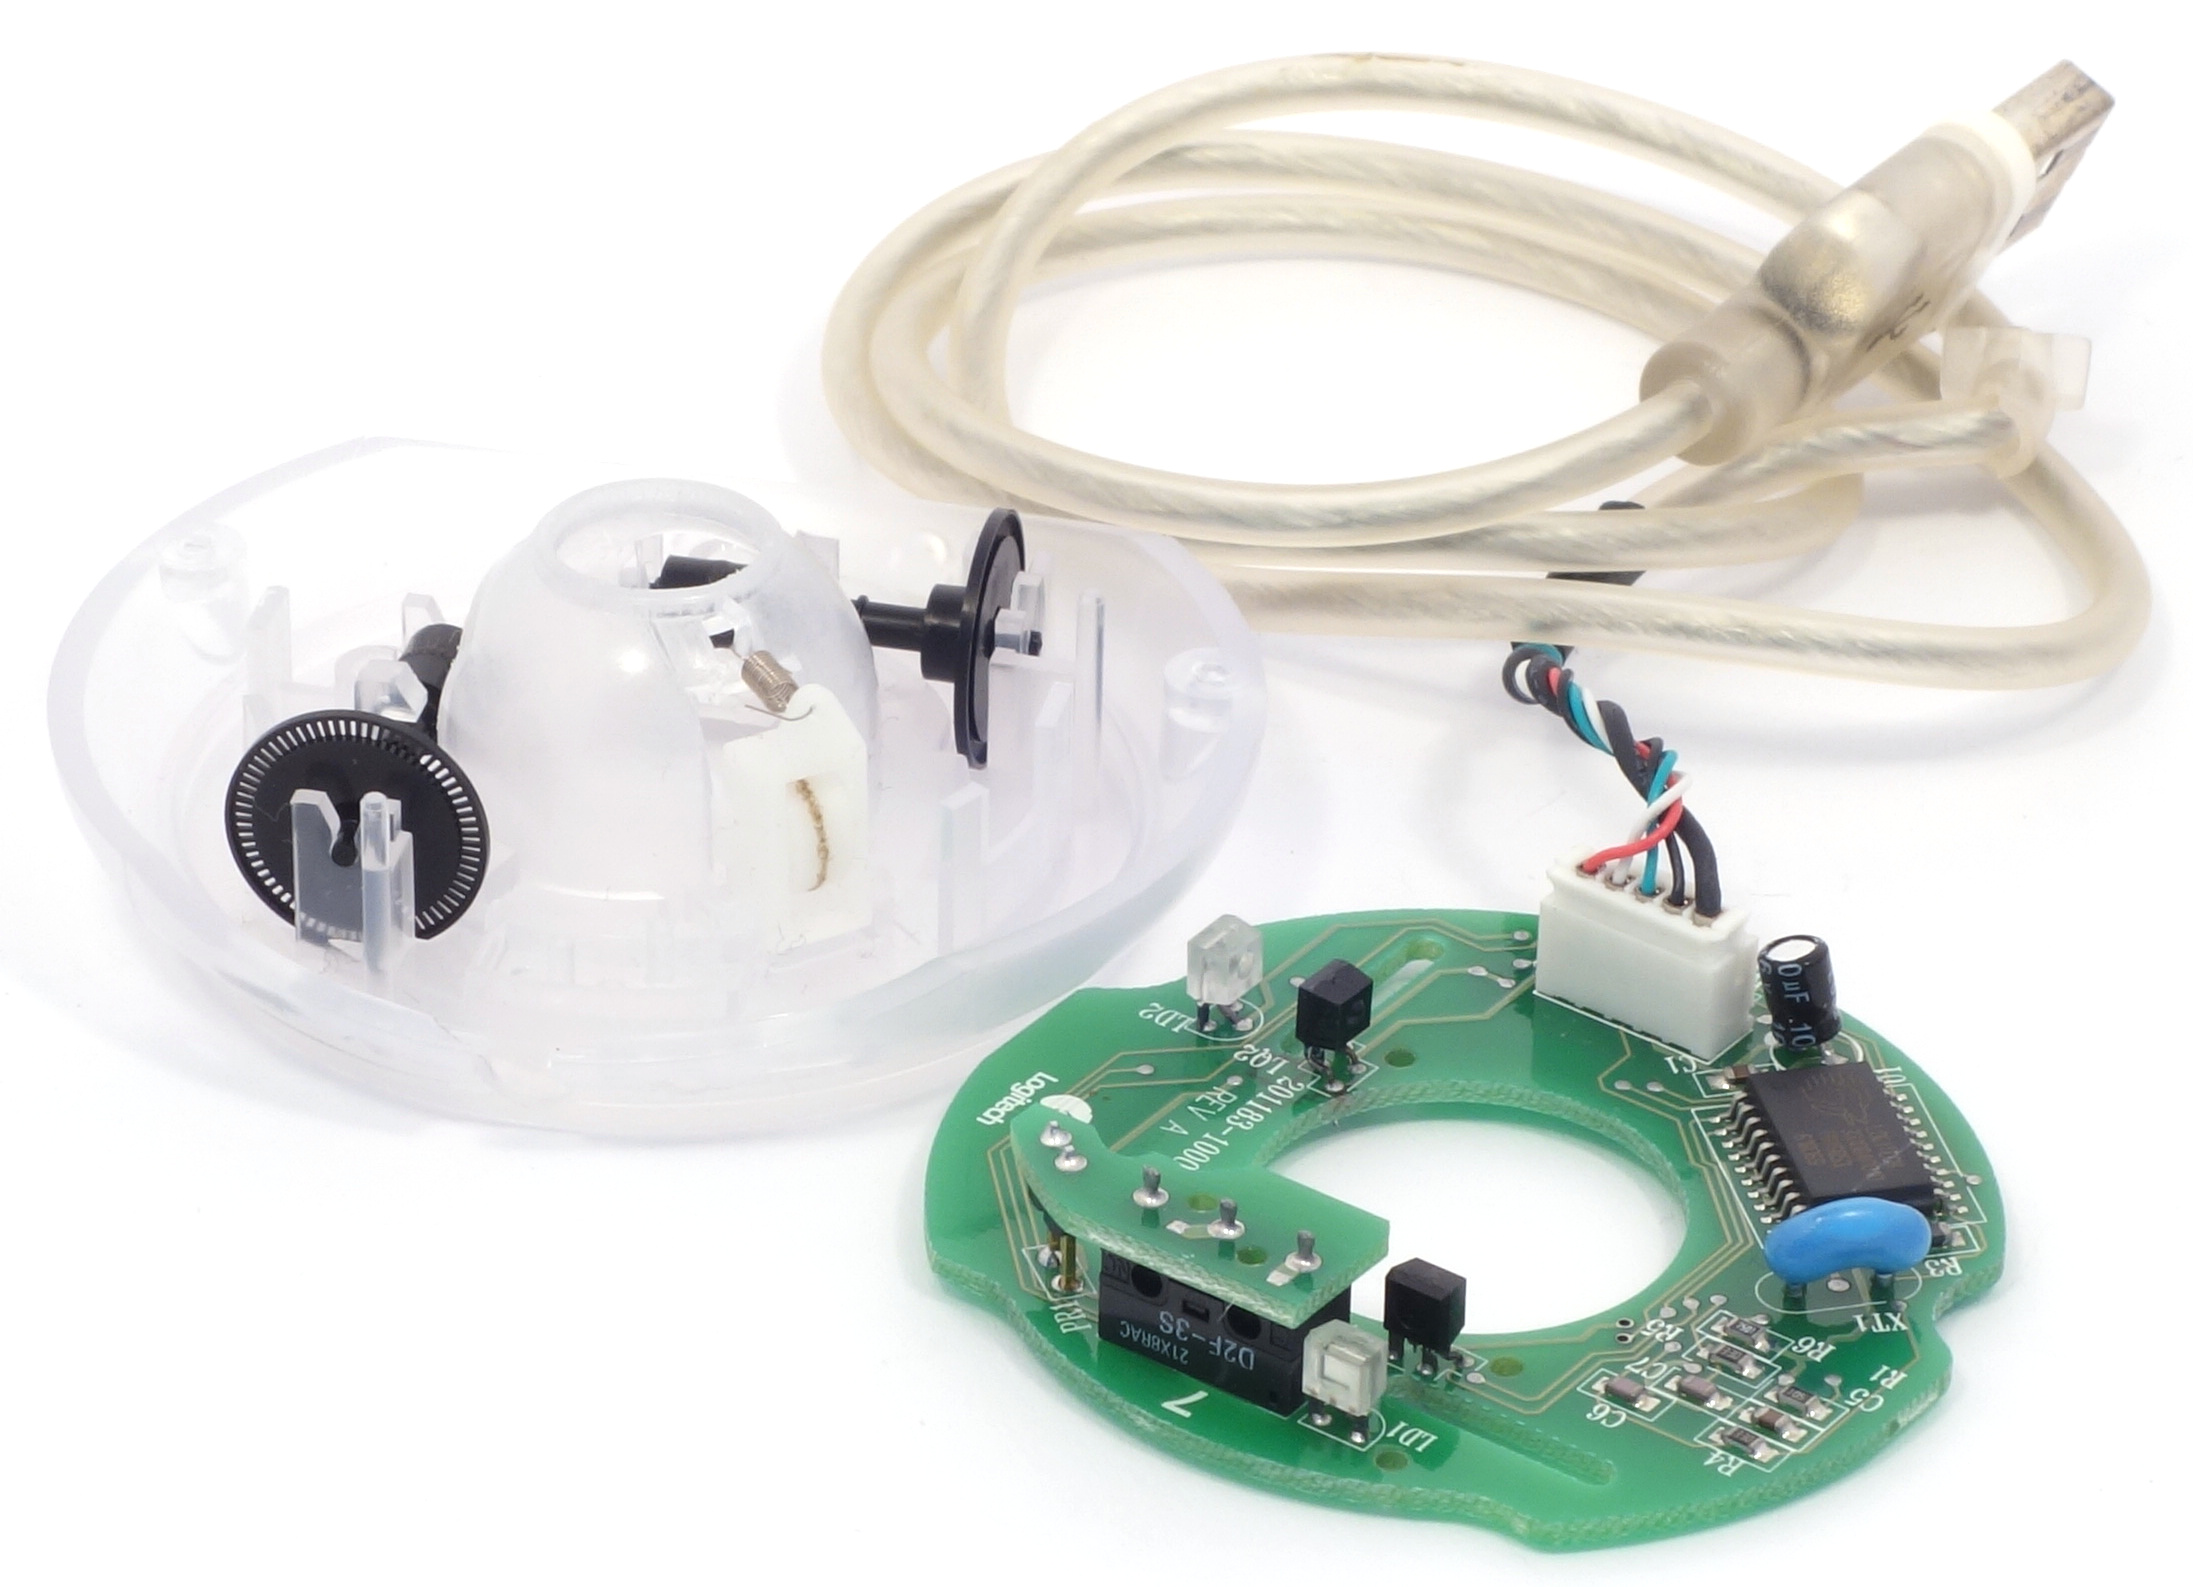
\includegraphics[scale=0.6]{1998_apple_puck/apple62.jpg}
    \caption{Apple Puck Mouse disassembled}
    \label{fig:inside}
\end{figure}

Mouse internals are shown on figure  \ref{fig:inside}. It is a typical opto-mechanical device.

\begin{thebibliography}{9}

    \bibitem {Apple} An ode to the puck, Apple's first USB mouse "--- \url{https://thehouseofmoth.com/an-ode-to-the-puck-apples-first-usb-mouse/} 
    \bibitem{icatch} The iCatch Mouse Adapter \url{https://web.archive.org/web/20001024170633/http://www.macsensetech.com:80/Product/iCatch.html}
\end{thebibliography}

\end{document}
